\clearpage

\section{CAPEX}\label{Heuristic_CAPEX}
\begin{tcolorbox}	
\begin{tabular}{p{2.75cm} p{0.2cm} p{10.5cm}} 	
\textbf{Student Name}  &:& Pedro Coelho    (March 01, 2018 - )\\
\textbf{Goal}          &:& Implement of the heuristic model to obtain the best possible CAPEX of a given network.
\end{tabular}
\end{tcolorbox}
\vspace{11pt}

The total CAPEX of a network, as it was already described in \ref{Capex}, is the sum between two differentiated costs. Firstly, the link cost depends on the link length, which has integrated components such as OLTs, transceivers and amplifiers and the node cost depends on the traffic intensity by each node.

In order to get the results for the heuristic approach, routing and grooming algorithms are used which try to obtain the most near optimal solution for the six cases detailed in this chapter. Then, it will be applied a cost report with all the detailed information about the costs of the network. The final CAPEX depends on the transport mode (opaque, transparent and translucent), possibility of the network having a dedicated 1+1 protection scheme or not and the network traffic (low - 0.5 Tbit/s, medium - 5 Tbit/s and high - 10 Tbit/s).

To calculate the total network cost it has to be considered the links cost and the nodes cost. The CAPEX value of a network, $C_C$, in monetary units (e.g. euros, or dollars), is calculated by the equation \ref{Capex_heuristic}.

\begin{equation}
C_C = C_L + C_N
\label{Capex_heuristic}
\end{equation}

Where

\begin{itemize}
\item{$C_L$				$\rightarrow$	Link cost in monetary units (e.g. euros, or dollars)}
\item{$C_N$				$\rightarrow$	Node cost in monetary units (e.g. euros, or dollars)}
\end{itemize}

On the first hand, the links' cost, $C_L$, in monetary units (e.g. euros, or dollars), is calculated by the equation \ref{Capex_Link_heuristic}. If the length of the link is longer, the resulting costs will be higher due to of the necessity of having more components which carry all the traffic from all origin nodes to all destination nodes.

\begin{equation}
C_L = \sum_{i=1}^N \sum_{j=i+1}^N L_{ij} \left( 2 \gamma_0^{OLT} + 2 \gamma_1^{OLT} \tau W_{ij} + N^R_{ij} c^R \right)
\label{Capex_Link_heuristic}
\end{equation}

Where

\begin{itemize}
\item{$i$               $\rightarrow$   Index for start node of a physical link}
\item{$j$               $\rightarrow$   Index for end node of a physical link}
\item{$N$				$\rightarrow$	Total number of nodes, N $\in \mathbb{N}$}
\item{$L_{ij}$			$\rightarrow$	Binary variable indicating if link between the nodes $i$ and $j$ is used, $L_{ij} \in {0, 1}$}
\item{$\gamma_0^{OLT}$	$\rightarrow$	OLT cost in monetary units (e.g. euros, or dollars)}
\item{$\gamma_1^{OLT}$	$\rightarrow$	Transponder cost in monetary units (e.g. euros, or dollars)}
\item{$\tau$		    $\rightarrow$	Line bit-rate}
\item{$W_{ij}$          $\rightarrow$   Number of optical channels in link $i$ $j$}
\item{$N^R_{ij}$    	$\rightarrow$	Number of optical amplifiers in link $i$ $j$}
\item{$c^R$				$\rightarrow$	Optical amplifiers cost in monetary units (e.g. euros, or dollars)}
\end{itemize}

The line bit-rate that is used in this report has the value of 100. It represents the separation between regeneration stages in km.

On the other hand, the nodes' cost, $C_N$, in monetary units (e.g. euros, or dollars), is calculated by the equation \ref{Capex_Node_heuristic}.

\begin{equation}
C_N = C_{EXC} + C_{OXC}
\label{Capex_Node_heuristic}
\end{equation}

Where

\begin{itemize}
\item {$C_{EXC}$        $\rightarrow$   Electrical node cost in monetary units (e.g. euros, or dollars)}
\item {$C_{OXC}$        $\rightarrow$   Optical node cost in monetary units (e.g. euros, or dollars)}
\end{itemize}

\vspace{11pt}
As all the nodes have an electrical part and an optical part, so it is necessary to calculate both with their respective formulas and sum the results.

The electrical nodes' cost, $C_{EXC}$, in monetary units (e.g. euros, or dollars), is given by the equation \ref{Capex_Node_EXC_heuristic}.

\begin{equation}
C_{EXC} = \sum_{n=1}^{N} N_{exc,n} \left( \gamma_{e0} + \sum_{c=-1}^B \gamma_{e1,c} P_{exc,c,n} \right)
\label{Capex_Node_EXC_heuristic}
\end{equation}

Where

\begin{itemize}
\item{$N$				$\rightarrow$	Total number of nodes, N $\in \mathbb{N}$}
\item{$N_{exc,n}$		$\rightarrow$	Binary variable indicating if node $n$ is used, $N_{exc,n} \in {0, 1}$}
\item{$\gamma_{e0}$ 	$\rightarrow$	EXC cost in monetary units (e.g. euros, or dollars)}
\item{$\gamma_{e1,c}$	$\rightarrow$	EXC port cost in monetary units (e.g. euros, or dollars) with bit-rate $B$ and with a given transceiver reach}
\item{$P_{exc,c,n}$	    $\rightarrow$	Number of ports of the electrical switch}
\item{$B$           	$\rightarrow$	A natural number corresponding to the maximum index of short-reach ports, see table below}
\end{itemize}

\begin{table}[H]
\centering
\begin{tabular}{|c|c|}
  \hline
  Index & Bit rate \\
 \hline\hline
  -1 & 100 Gbits/s line bit-rate (long-reach port) \\
  0 & 1.25 Gbits/s tributary bit-rate (short-reach port) \\
  1 & 2.5 Gbits/s tributary bit-rate (short-reach port) \\
  2 & 10 Gbits/s tributary bit-rate (short-reach port) \\
  3 & 40 Gbits/s tributary bit-rate (short-reach port) \\
  4 & 100 Gbits/s tributary bit-rate (short-reach port) \\
  \hline
\end{tabular}
\caption{Table with index and your corresponding bit rate}
\label{table_bitrate_heuristic}
\end{table}

The constitution of the electrical node part can be seen in the Integer Linear Programming section \ref{exc_design}.

Finally, the optical nodes' cost, $C_{OXC}$, in monetary units (e.g. euros, or dollars), is given by the equation \ref{Capex_Node_OXC_heuristic}.

\begin{equation}
C_{OXC} = \sum_{n=1}^{N} N_{oxc,n} \left( \gamma_{o0} + \gamma_{o1} P_{oxc,n} \right)
\label{Capex_Node_OXC_heuristic}
\end{equation}

Where

\begin{itemize}
\item{$N$				$\rightarrow$	Total number of nodes, N $\in \mathbb{N}$}
\item{$N_{oxc,n}$		$\rightarrow$	Binary variable indicating if node $n$ is used, $N_{oxc,n} \in {0, 1}$}
\item{$\gamma_{o0}$ 	$\rightarrow$	OXC cost in monetary units (e.g. euros, or dollars)}
\item{$\gamma_{o1}$ 	$\rightarrow$	OXC port cost in monetary units (e.g. euros, or dollars) }
\item{$P_{oxc,n}$	    $\rightarrow$	Number of ports of the optical switch}
\end{itemize}

The constitution of the optical node part can be seen in the Integer Linear Programming section \ref{oxc_design}.

To obtain the best possible value, it will be necessary to minimize the cost of the CAPEX mentioned above so that we can obtain the objective function \ref{Minimize_Heuristic_CAPEX}.

\begin{equation}
minimize \qquad \qquad C_C
\label{Minimize_Heuristic_CAPEX}
\end{equation}

After all the formulas needed to calculate the CAPEX of a network are demonstrated above, it is also essential to have pre-defined the costs of the network equipments. In the table \ref{table_cost_heuristic} it is shown the cost, in euros, of all the equipments with their symbols used in the respective formulas.\\

\begin{table}[H]
\centering
\begin{tabular}{|| c | c | c||}
 \hline
 Equipment & Symbol & Cost \\
 \hline\hline
 OLT without transponders & $\gamma_0^{OLT}$ & 15000 \euro \\
 Transponder & $\gamma_1^{OLT}$ & 5000 \euro/Gb \\
 Unidirectional Optical Amplifier & $c^R$ & 4000 \euro \\
 EXC & $\gamma_{e0}$ & 10000 \euro \\
 OXC & $\gamma_{o0}$ & 20000 \euro \\
 EXC Port for line ports & $\gamma_{e1,-1}$ & 1000 \euro /Gb/s\\
 EXC Port for ODU0 & $\gamma_{e1,0}$ & 8 \euro /Gb/s\\
 EXC Port for ODU1 & $\gamma_{e1,1}$ & 6 \euro /Gb/s\\
 EXC Port for ODU2 & $\gamma_{e1,2}$ & 3 \euro /Gb/s\\
 EXC Port for ODU3 & $\gamma_{e1,3}$ & 1.5 \euro /Gb/s\\
 EXC Port for ODU4 & $\gamma_{e1,4}$ & 1 \euro /Gb/s\\
 OXC Port & $\gamma_{o1}$ & 2500 \euro /porto \\
 \hline
\end{tabular}
\caption{Table with costs}
\label{table_cost_heuristic}
\end{table}

In the next page it is shown the heuristic algorithms approach used in the programming softwares Eclipse and Net2Plan. We can see the most important aspects to take into account by using these algorithms and the arguments and differences used in each of them. The argument "t" \space refers to the transport mode.

\begin{figure}[H]
\centering
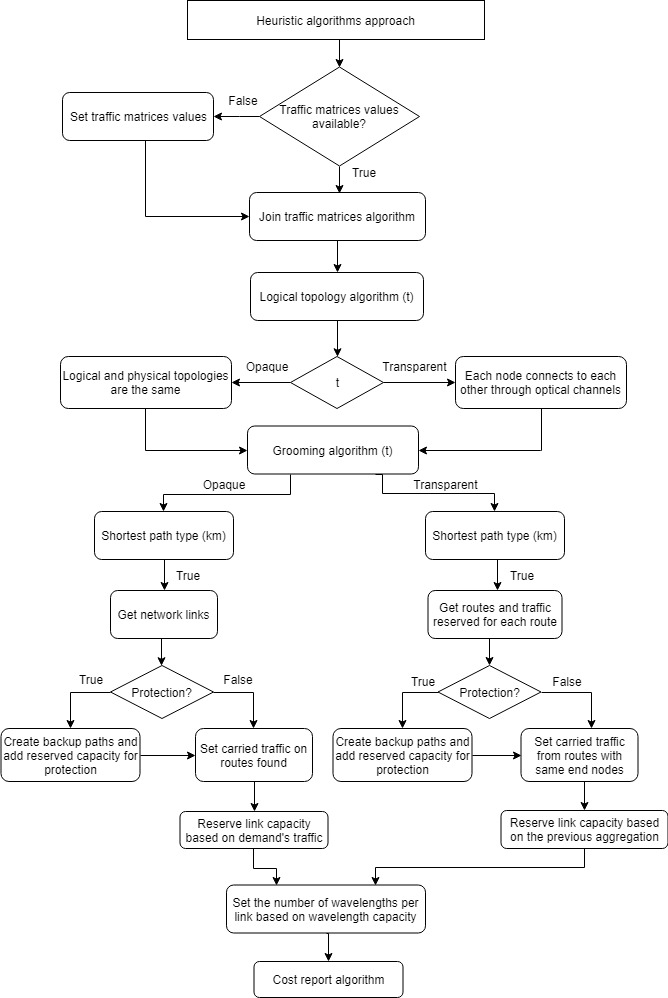
\includegraphics[width=15cm]{sdf/heuristic/figures/heuristic_fluxogram}
\caption{Fluxogram with heuristic algorithms approach.}
\label{fluxogram_heuristic}
\end{figure}
